% !TEX encoding = UTF-8
% !TEX TS-program = pdflatex
% !TEX root = ../Tesi.tex
% !TEX spellcheck = it-IT

%************************************************

%************************************************
%Il sistema Url2vec si propone come alternativa alle metodologie di clustering di siti web basate sul contenuto testuale delle pagine~\cite{Rajaraman11}. 
I grafi possono essere utilizzati per modellare innumerevoli fenomeni reali, da quelli scientifici a quelli sociali. Questi rappresentano le entità non come singole unità descritte appieno dalle loro caratteristiche, ma piuttosto dai collegamenti che intercorrono tra di esse. Queste ''relazioni'' codificano la maggior parte delle informazioni latenti in un grafo, caratterizzandolo in maniera univoca.

In questa tesi si approfondiscono tecniche e metodologie per le estrazione di queste informazioni dal grafo del Web, più precisamente di un sito Web, indirizzate alla divisione delle pagine in cluster omogenei. Le pagine Web tuttavia non sono divisibili in classi ben definite, non ci sono informazioni esplicite che rappresentano univocamente i professori, gli studenti o i corsi. Data questa assenza, non è possibile generare un modello accurato di classificazione. Si è rivelato necessario risolvere il problema con un latro approccio.

A dispetto della diversità delle pagine Web nella rete, quelle che risiedono all'interno di una particolare organizzazione, spesso, condividono una certa struttura. Questa può essere appresa attraverso l'analisi del peso, della densità o della direzione degli hyperlink presenti nelle pagine Web, ovvero gli archi del grafo costruito su di esse. Ad esempio, il sito Web di un dipartimento di informatica conterrà pagine riguardanti i docenti, gli studenti, i corsi, la ricerca che saranno accessibili attraverso determinati \textit{percorsi} del grafo. L'analisi dei grafi comporta anche degli svantaggi, gli algoritmi della teoria dei grafi sono NP-completi \cite{Garey}, e questo non può essere trascurato considerando le dimensioni del Web. Nella metodologia presentata viene proposta l'alternativa di apprendere rappresentazioni vettoriali dei vertici all'interno del grafo, utilizzandole insieme alle informazioni estratte dal contenuto di una pagina Web, così da processare vettori linearmente indipendenti. Queste rappresentazioni vettoriali sono apprese attraverso la generazione di percorsi attraverso gli archi del grafo, creando delle sequenze di vertici che saranno trattate come frasi, dove le parole sono pagine Web. 


\subsection{NLP nel Web: URL Embedding}
In questo modo è possibile sfruttare i recenti sviluppi nel campo del Word Embedding. Questi algoritmi riescono a considerare sempre più fattori e restituire vettori sempre più accurati. Vengono incluse informazioni riguardanti il contesto di una parola, ovvero gli altri termini contenuti nella frase in cui compare la parola analizzata. Nel Web questo implica considerare le pagine ''più vicine'', ovvero le pagine che puntano o sono puntate direttamente dalla pagina in esame, privilegiando quelle che hanno più collegamenti con questa. Questa informazione riesce ad estrarre le informazioni latenti nella struttura del sito, ed a raggruppare le pagine similmente ad un algoritmo di partizionamento di un grafo. Queste informazioni hanno rivelato proprietà peculiari quando applicate su grandi testi. Il caso più noto e controverso è quello delle analogie. 

È stato osservato che correlazioni nascoste possono trovarsi nella differenza tra coppie di vettori~\cite{Mikolov13}, come nel caso di parole simili ma con leggere differenze come il genere o il numero, infatti esse appaiono in frasi tendenzialmente simili, ma con delle piccole differenze. In questo caso l'informazione può essere interpretata come il genere o il numero.
\\\\
Informazioni simili possono essere trovate anche nel campo del Web. È ormai consolidata la questione dell'autorità di alcune pagine~\cite{Kleinberg99} e di come queste abbiano un maggior numero di link in entrata. Alcune pagine tuttavia saranno accessibili prevalentemente attraverso alcuni percorsi e si troveranno quindi in un contesto con elementi simili. Il problema resta dare un senso a queste correlazioni ed un significato utilizzabile. Nello sviluppo di Url2vec, tuttavia, sono emerse corrispondenze abbastanza naturali, come le pagine dei professori con i relativi corsi insegnati o i laboratori di afferenza. 

Queste relazioni sono dovute al fatto che il grafo di un sito Web è fortemente connesso, ma la maggior parte delle volte in cui appare un determinato corso di studio appare anche il relativo docente e viceversa. 

\subsection{Differenza tra parole ed URL}
La sola analisi delle sequenze comunque può risultare limitata. Le pagine Web non sono parole, ad esse è associata un ulteriore informazione, ovvero il contenuto testuale. Questa proprietà si è rivelata molto utile, infatti combinando le informazioni ricavate dall'esame di tutti e due gli aspetti, il grado di accuratezza del processo di clustering è salito in modo significativo. Il contenuto di una pagina infatti fornisce informazioni fondamentali su di essa, ma queste possono variare significativamente anche tra pagine considerate dello stesso tipo, presentando ad esempio una diversa distribuzione dei termini. Analizzando la struttura connessa delle pagine Web, si è cercato costruire delle rappresentazioni più significative.
%https://www.ideals.illinois.edu/bitstream/handle/2142/45402/Timothy_Weninger.pdf?sequence=1}
%The parallel path framework for entity discovery on the Web
Saper sfruttare tale struttura può agevolare notevolmente i task di Web Mining. Esso infatti estrae conoscenza strutturata e facilmente processabile.

%A partire da questo punto stai per descrivere il COME hai realizzato il tuo sistema, peccato che manca il COSA, ossia cosa fa il tuo sistema, cosa hai fatto di interessante, in che modo il tuo sistema è capace di superare delle open challenges, ect.
Nelle sottosezioni che seguono si descrive il sistema realizzato, oltre che le tecniche e gli algoritmi utilizzati per la realizzazione degli obiettivi preposti.\\
Sono state realizzate tre macro componenti.
\begin{itemize}
\item \textit{Crawling delle pagine Web}. Questo è regolato da alcuni parametri che rendono il processo flessibile e altamente modificabile.
\item \textit{Costruzione del Dataset}, ovvero la strutturazione delle informazioni ottenute nel processo precedente, secondo alcuni criteri necessari per le successive elaborazioni.
\item \textit{Clustering delle pagine Web} attraverso la combinazione dell'analisi del contenuto testuale e delle relazioni tra le pagine.
\end{itemize}

\section{Web Crawling per l'estrazione dei dati}
\label{crawling}
Le proprietà che caratterizzano le pagine Web rendono complicato il processo di estrazione di informazioni, soprattutto nel caso in cui i contenuti vengono generati dinamicamente.

\begin{figure}[htb]
	\centering
	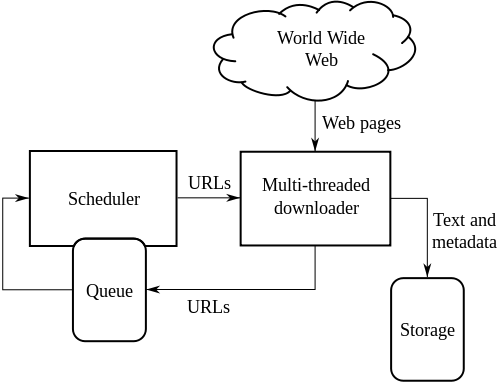
\includegraphics[width = 100mm]{crawlerarch.png}
	\caption{Architettura di un web crawler}
	\label{crawlerarch}
\end{figure}

Un Web crawler, chiamato anche web spider o web robot, è un componente software. I suoi obiettivi principali sono:
\begin{itemize}
\item raccogliere il più velocemente ed efficientemente possibile pagine utili, insieme alla struttura ad hyperlink che le collega;
\item copiare tutte le pagine che visita per elaborazioni future, per poi indicizzarle cosi che gli utenti possano trovarle più velocemente;
\item validare gli hyperlink e il codice HTML;
\item eseguire il Web Scraping delle pagine Web.
\end{itemize}

Esso esplora una pagina alla volta, analizandone la struttura e gli hyperlink contenuti. Questi sono immagazzinati nella ''frontiera'' che inizialmente vuota, conserva tutte le pagine ancora da esplorare. L'ordine di esplorazione e le politiche di filtraggio degli hyperlink possono variare in base al risultato desiderato. 

\begin{algorithm}[H]
\caption{Crawling BFS}
\begin{algorithmic}

	\State $url\gets homepage$;	\Comment{Pagina da cui iniziare}
	\State $queue\gets empty$ \Comment{Coda per la BFS}
	\State $analyzedVertex.add(url)$;	\Comment{Insieme di url già visitati}
	\State $maxDepth url$;	\Comment{Massima profondità di esplorazione}
 	
 	\vspace*{+0.5cm}
 	
	\State \textbf{Begin}
	\While{$queue \neq empty$} 
		\State $urlToAnalyze\gets queue.dequeue()$
		
		\If{$urlToAnalyze.depth \leq maxDepth$}
			\State $outlinks \gets urlToAnalyze.getOutlinks()$
		\Else
			\State $urlToAnalyze$
		\EndIf
		\If{$outlinks \neq null$}
			\State $outlinks \gets urlToAnalyze.getOutlinks()$
			\State $analyzedVertex.add(outlinks)$
			\State $serialize(urlToAnalyze)$
			\For{\textbf{each} link in outlinks}
				\State $serialize(link)$
				\State $queue.enqueue(link, urlToAnalyze + 1)$
			\EndFor
		\EndIf
		
	\EndWhile
	\State \textbf{End}
\end{algorithmic}
\end{algorithm}

\subsection{Proprietà del web crawler}
Nel processo di Crawling, data la natura non strutturata del Web, è necessaria l'applicazione di numerose tecniche e metodologie per un corretto funzionamento.

\subsubsection{Normalizzazione degli URL}
Il termine di normalizzazione, chiamato anche canonicalizzazione di URL, si riferisce al processo di modifica e standardizzazione di un URL in una maniera consistente, ad esempio alcuni siti Web mettono a disposizione gli stessi file o i medesimi contenuti attraverso URL differenti. 
\\\\
\texttt{http://domain.com/products/page.php?product=smartphone}
\\
\texttt{http://domain.com/products/smartphone.php}
\\\\
\texttt{http://www.domain.edu/courses}
\\
\texttt{http://www.domain.edu/courses/index.html}
\\\\
Le due coppie di URL nell’esempio puntano agli stessi contenuti. Altri casi sono URL che differscono solo per il protocollo (''\texttt{http://}'' o ''\texttt{https://}'') o l'omissione della stringa ''\texttt{www}''. Effettuando la normalizzazione, si sceglie un URL come formato di riferimento per accedere ad un determinato contenuto. Ci sono diversi tipi di normalizzazione che possono essere usati, come la conversione in minuscolo, rimuovere i ''.'' e ''..'' portando gli URL relativi ad URL assoluti, aggiungere slash finali al componente di percorso non vuoto.
\\\\
Una soluzione consiste nella creazione di un dizionario che ha come chiavi gli hashcode del contenuto testuale delle pagine e come valori una lista di tutti i diversi URL che hanno quel contenuto. In questo modo si riduce il problema ad una sola operazione così da annullare le relazioni e i vari di pattern da scovare nall'analisi degli URL per capire se sono la stessa pagina o meno. 

\subsubsection{Ricerca all'interno dello stesso dominio}
Per estrarre informazione e per il successivo processo di clustering delle pagine web, è necessario che le pagine estratte si riferiscano allo stesso dominio, o in altri termini, che appartengano allo stesso sito web.
\\
Questo viene effettuato per sfruttare la struttura gerarchica del dito web rivolto principalmente riuscire a  raccogliere le informazioni nascoste nel grafo e sopratutto negli hyperlink.

\subsubsection{Dimensione della ricerca}
Anche limitando la ricerca ad un solo dominio, la dimensione delle pagine da esplorare, e quindi la grandezza della frontiera, può aumentare considerevolmente o addirittura portare il processo di crawling a divergere.

\begin{figure}[htb]
	\centering
	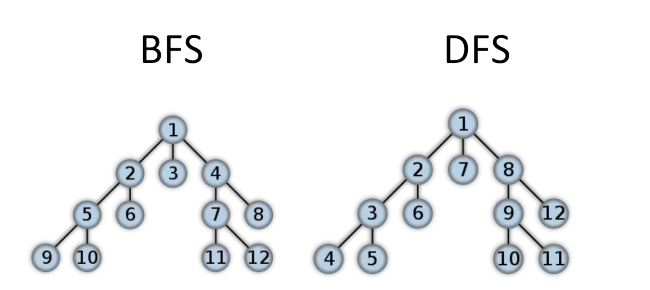
\includegraphics[width = 100mm]{breadthdepth.png}
	\caption{Differenze tra ricerca in ampiezza e ricerca in profondità}
	\label{breadthsearch}
\end{figure}

È stata utilizzata una ricerca in ampiezza con un limite variabile di profondità. Ponendo un limite all'esplorazione del grafo delle pagine si garantisce la la terminazione del processo di crawling e utilizzando una ricerca in ampiezza si dà priorità alle pagine vicine al nodo radice (comunemente l'homepage). Questa scelta è stata dettata anche dal cercare di evitare le cosiddette ''spider traps''. Queste sono dei meccanismi utilizzati, intenzionalmente o involontariamente, dai server oggetto di crawling, che possono portare ad una generazione dinamica e potenzialmente infinita in URL univoci, e quindi considerati come pagine diverse. Questo può essere evitato non aggiungendo alla frontiera URL che contengono il carattere ''?'', ma questo non è sempre efficace.
\\\\
Inoltre è stato osservato che nei siti web entity-oriented, le informazioni ricercate si trovano quasi sempre nei primi livelli di gerarchia \cite{He13}.

\subsubsection{Restrizione dell'esplorazione}
La restrizione può essere effettuata sulle pagine da esplorare o dalla frequenza di richieste che è possibile effettuare.
\\\\
Il robots exclusion protocol è uno standard che consiste in un file (robots.txt), posto alla radice della gerarchia di un sito Web. In pratica, il file indica le regole utilizzate dai crawler per applicare restrizioni di analisi sulle pagine di un sito web. 
\\\\
Molte volte i crawler non sono ben accetti, in quanto possono rallentare pesantemente la navigazione. Se server effettua dei controlli sulle richieste ricevute e queste hanno una frequenza troppo elevata o seguono uno schema riconducibile ad una macchina queste possono essere ignorate. Può capitare che richieste continue e non curanti delle restrizioni imposte portino a bandire l'indirizzo IP del servizio trasgressore.\\
Per evitare tali conseguenze è opportuno seguire una certa etica nell'operazione di crawling.

\subsection{Estrazione delle liste}
\label{liste}
Riuscire a strutturare dati non strutturati può rivelarsi ostico. Molti tentativi, più o meno efficaci, sono stati effettuati a tale proposito.
\\
In questa tesi uno degli obiettivi è stato quello di prendere in considerazione i collegamenti all'interno delle pagine web, seguendo i percorsi generati dalla concatenazione di più hyperlink. Questa scelta è stata effettuata sulla base dei recenti progressi nel campo del natural language processing (NLP)~\cite{Turian10}. Esplorando la struttura del grafo del web, data la forte connessione che esiste fra i suoi nodi, estrarre informazione può rivelarsi un operazione tutt'altro che banale. 
\\\\
È stato introdotto il concetto di \textbf{lista}. 
Per permettere una migliore visualizzazione dell’informazione descritta, quasi tutte le pagine web vengono formattate utilizzando regole CSS. Di conseguenza, per poter effettuare correttamente questo task, bisogna prima elaborare la pagina Web con tutte le informazioni grafiche sui nodi HTML e solo successivamente si può procedere alla loro estrazione. Grazie alle informazioni ricavate dall’HTML della pagina Web e dalla posizione e dimensione dei singoli nodi, è possibile stabilire una struttura gerarchica ad albero dei nodi che la compongono. Questa struttura gerarchica ad albero permette di scoprire i record, ovvero dati strutturati (ad esempio provenienti da database) che sono allineati orizzontalmente, verticalmente e anche strutturalmente (elementi HTML ul, li, . . . ); permette quindi di individuare dei gruppi di record, ovvero delle liste di record.
\\
L’individuazione delle liste di raggiungere pagine che contengono elementi simili a quelli contenuti nella pagina che si sta visualizzando. 
In questo modo le pagine dovrebbero essere accessibili solo attraverso percorsi predeterminati e non in maniera fortemente connessa. I nodi e gli archi risultanti risultano così un sottoinsieme di quelli originali.

\section{Costruzione del Dataset}
I dati estratti nel processo vanno organizzati e ampliati in modo da garantire l'accesso e l'elaborazione in maniera agevole.
\\
Il processo di crawling restituisce il grafo delle pagine web e il contenuto testuale di ogni pagina esplorata, a queste va aggiunta la generazione delle sequenze attraverso la teoria dei \textit{Random Walk}, come spiegato in \ref{rwsection}. Inoltre per un minor spreco di risorse si è optato per la conversione degli URL in codici, ovvero una associazione univoca fra un URL ed un codice (e.g. un numero) molto più corto, così da risparmiare tempo di elaborazione e spazio di archiviazione.

\subsection{Random Walk}
\label{rwsection}
Per la generazione delle sequenze è stato utilizzata la teoria dei \textit{Random Walk}. In matematica, un Random Walk è la formalizzazione dell'idea di prendere passi successivi in direzioni casuali. Matematicamente parlando, è il processo stocastico più semplice, il processo markoviano. Qui sono utilizzati per ricavare percorsi pseudo casuali da attraversamento del grafo del web per ottenere sequenze di URL collegati semanticamente.
\\\\
In una passeggiata aleatoria monodimensionale si studia il moto di una particella puntiforme vincolata a muoversi lungo una retta nelle due direzioni consentite. Ad ogni movimento essa si sposta (a caso) di un passo a destra (con una probabilità fissata $\ p$) o a sinistra con una probabilità $\ 1-p$, ed ogni passo è di lunghezza uguale e indipendente dagli altri.
\begin{figure}[htb]
	\centering
	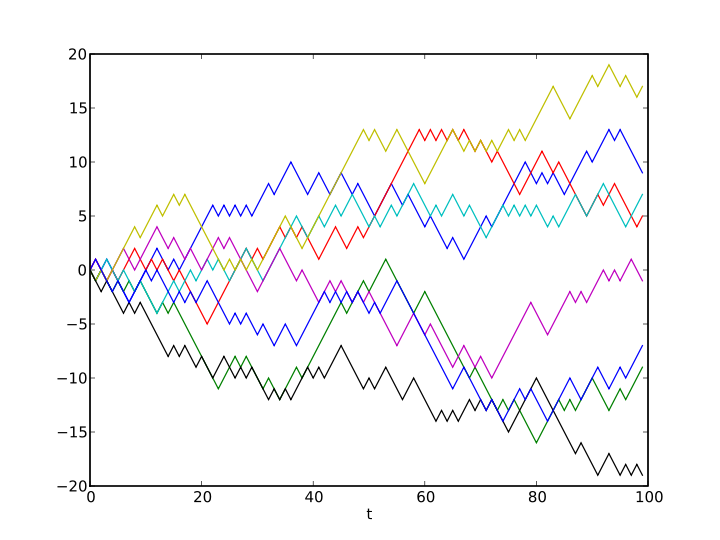
\includegraphics[width = 100mm]{randomwalkonedim.png}
	\caption{Rappresentazione visuale di 8 random walk monodimensionali. }
	\label{englishchinese}
\end{figure}
\\\\
In una passeggiata aleatoria bidimensionale si studia il moto di una particella vincolata a muoversi sul piano spostandosi casualmente ad ogni passo a destra o a sinistra con probabilità $\frac{1}{2}$, verso l'alto o verso il basso con probabilità $\ p=\frac{1}{2}$. In pratica ad ogni passo può compiere un movimento lungo una delle quattro diagonali con probabilità $\frac{1}{4}$. Ci si chiede con che probabilità la particella tornerà al punto di partenza.
\begin{figure}[htb]
	\centering
	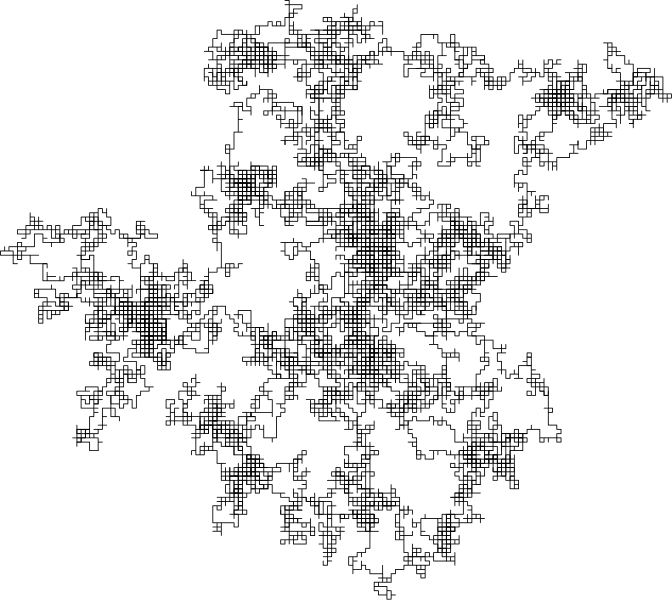
\includegraphics[width = 100mm]{randomwalktwodim.png}
	\caption{Rappresentazione visuale di un random walk di 25.000 passi su due dimensioni. }
	\label{englishchinese}
\end{figure}
\\\\
Queste passeggiate aleatorie possono trovare effettivi riscontri in natura come il traiettoria percorso da una particella in un liquido o in un gas, il tragitto di un animale affamato o anche il prezzo di un titolo fluttuante o la situazione finanziaria di un giocatore d'azzardo. Tutti questi esempi possono essere espressi come random walk, anche se in natura potrebbero non essere veramente casuali.
\\\\
Un popolare modello di random walk è quello su un reticolo regolare, dove ad ogni passo si segue un determinato percorso basandosi su una qualche distribuzione di probabilità. Nel caso più semplice si può solo “saltare” sul sito vicino. In un semplice random walk simmetrico in un reticolo localmente finito, le probabilità di saltare su ognuno dei siti vicini è la stessa.
\\\\
Per definire un random walk formalmente, prese indipendenti variabili casuali $ Z_1, Z_2, Z_3, $ \dots dove ogni variabile è o 1 o -1, con una probabilita del 50\% per ognuno dei due casi, e dato 
\begin{equation}
  S_0 = 0
\end{equation}
\begin{equation}
  S_n = \sum_{j=1}^{n} Z_j
\end{equation}
  
la serie $\left \{ S_n \right \} $ è chiamata random walk semplice in $\mathbb{Z}$.
\\\\
Si consideri un attraversatore casuale della rete (random surfer) che, partendo da un pagina web, esegue un passo alla volta in questo modo: ad ogni iterazione, dalla pagina corrente, procede verso una pagina a caso tale che esiste un link che dalla pagina corrente punta a questa.
\\\\
Procedendo da pagina a pagina, visiterò alcuni nodi, più spesso di altri; intuitivamente, saranno nodi con molti link entranti da altri nodi frequentemente visitati. Ci sono alcuni problemi. Che succede se si arriva ad una pagina che non ha link in uscita? In questo caso è necessario introdurre un’altra operazione: il teletrasporto. In questa operazione l’attraversatore casuale salta dal nodo corrente ad un qualsiasi altro nodo sulla rete.
Se $N$ è il numero totale dei nodi nel grafo, l’operazione di teletrasporto porta l’attraversatore verso ogni nodo con probabilità $\frac{1}{N}$. Potrebbe anche trasportarsi sulla posizione corrente con probabilità di $\frac{1}{N}$. Questa operazione è chiamata quando si arriva ad un non senza nodi in uscita o con una probabilità$\ d$ data, con$\ 0 < d < 1$.


\subsection{Generazione delle sequenze}
Le sequenze rappresentano un percorso che un attraversatore casuale della rete seguirebbe cliccando su un hyperlink a caso fra tutti quelli disponibili nella pagina corrente (o eventualmente nelle liste). Questi percorsi, chiamati \textbf{Random Walk} (o passeggiate aleatorie), sono stati largamente utilizzati in molti algoritmi sui grafi e sul Web~\cite{aldous14} in quanto buone approssimazioni di comportamenti casuali. Il problema di questa tecnica applicata al Web si presenta quando l'attraversatore casuale arriva ad una pagina priva di hyperlink. La soluzione più diffusa consiste nell'effettuare un ''salto'' verso una qualsiasi altra pagina quando non ci sono outlink da seguire. 
\\\\
Qui il problema non si pone, in quanto le sequenze generate hanno una lunghezza fissata prima dell'esecuzione e se la generazione dovesse bloccarsi, la sequenza risultante sarà solo più piccola. Questa scelta è dovuta dal fatto che l'informazione cercata scaturisce da percorsi reali di navigazione e non necessita una lunghezza obbligatoria da rispettare, in quanto le sequenze possono essere viste come frasi di un testo, dove le parole sono gli URL.
\\\\
Per motivi di sperimentazione sono stati implementati tre tipi diversi di Random Walk, utilizzabili modificando i parametri di esecuzione dell'algoritmo.



\begin{algorithm}[H]
\caption{Generazione delle sequenze}
\begin{algorithmic}

	\State $numRandomWalks$;	\Comment{Numero di Random Walk da generare}
	\State $lengthRandomWalks$ \Comment{Lunghezza dei Random Walk}
 	
 	\vspace*{+0.5cm}
 	
	\State \textbf{Begin}
	\State $node \gets \Call{randomnode}{}$
	\For{$i \gets 0 \to numRandomWalks$} 
		\State $sequence.add(node)$
		
		\While{$sequence.length \leq lengthRandomWalks$}
			\If{$node.hasOutlinks()$}
				\State $node \gets node.getOutlinks(RandomIndex)$
				\State $sequence.add(node)$
			\Else
				\State $break$
			\EndIf
		\EndWhile
		\State $serialize(sequence)$
		
	\EndFor
	\State \textbf{End}
\end{algorithmic}
\end{algorithm}


\subsubsection{Random Walk standard}
Questo è il caso standard, ovvero si parte da un nodo casuale del grafo e si segue ogni volta un arco a caso fra quelli disponibili, fino al raggiungimento della lunghezza prefissata o all'impossibilità di proseguire.
\\
Da notare che questo processo e il precedente non sono completamente separati, in quanto la scelta di un nodo casuale e la consecutiva traiettoria, possono portare all'esplorazione di pagine non precedentemente visitate. È quindi necessario mantenere aggiornato il grafo immagazzinato.
\begin{figure}[htb]
	\centering
	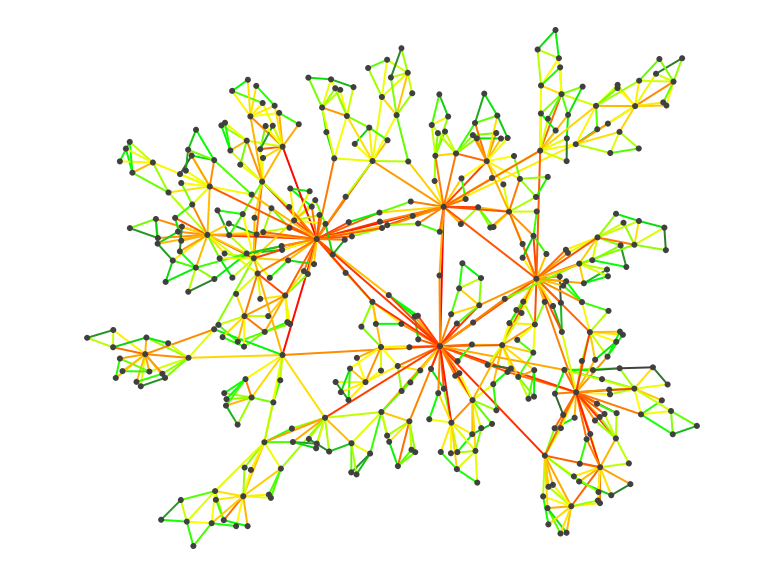
\includegraphics[width = 100mm]{randomWalkongraph.png}
	\caption{Random walk sul grafo. }
	\label{englishchinese}
\end{figure}
\subsubsection{Random Walk con partenza fissa}
Qui l'unica differenza consiste nel punto di partenza del cammino. Infatti si può partire in un nodo prefissato del grafo (generalemnte l'homepage di un sto web), in modo da esplorare più percorsi possibili avente quel nodo come origine.

\subsubsection{Random Walk attraverso le Liste}
Qui invece si può seguire uno dei due approcci precedenti, ma con il vincolo delle liste, quindi limitando la camminata ad un sottoinsieme di quella precedente.

\subsection{Esempio di Dataset}
Di seguito sono elencati file generati nel processo di crawling e di generazione delle sequenze. Gli esempi riportati di seguito sono stati ottenuti analizzando il sito del dipartimento di informatica di Urbana, IL: \texttt{www.cs.illinois.edu}

\subsubsection{urlsMap.txt}
Contiene la associazioni fra gli URL e il relativo codice identificativo. Questo è dovuto dalle ragioni spiegate in precedenza, ovvero ridurre i tempi di elaborazione e spazio di archiviazione. 
\\\\
\texttt{
http://cs.illinois.edu,3\\
http://cs.illinois.edu/prospective-students,4\\
http://cs.illinois.edu/current-students,5\\
http://cs.illinois.edu/courses,6\\
http://cs.illinois.edu/alumni,7\\
http://cs.illinois.edu/research,8\\
http://cs.illinois.edu/news,9\\
http://cs.illinois.edu/partners,10\\
http://cs.illinois.edu/about-us,11\\
. . .\\
}
\subsubsection{vertex.txt}
Contiene il contenuto testuale di ogni pagina esplorata. Ogni riga è quindi formata da il codice identificativo di un URL e il relativo contenuto.
\\\\
\texttt{
1	department of computer science at illinois engineering at ...\\
2	prospective students department of computer science at ...\\
3	current students department of computer science at ...\\
4	courses department of computer science at illinois ...\\
5	alumni department of computer science at illinois ...\\
6	research department of computer science at illinois    ...\\
7	news department of computer science illinois engineering ...\\
8	partners department of computer science at illinois ...\\
9	about us department of computer science at illinois ...\\
. . .\\
}
\subsubsection{edges.txt}
Questo è il file principale per la generazione delle sequenze, qui sono immagazzinate tutte le relazioni fra le pagine, ovvero gli archi che le collegano. 
\\\\
\texttt{
1	1\\
1	2\\
1	3\\
1	4\\
1	5\\
1	6\\
1	7\\
1	8\\
1	9\\
. . .\\
}
\subsubsection{sequencesIDs.txt}
Contiene le sequenze generate. I codici relativi alle pagine web sono separati da '' -1 '' e la linea finisce con un '' -2 ''. Da notare che sono riportate le sequenze che partono da un nodo casuale del grafo.
\\\\
\texttt{
137 -1 2 -1 27 -1 8 -1 52 -1 53 -1 8 -1 8 -1 10 -1 13 -1 -2\\
506 -1 5 -1 14 -1 11 -1 6 -1 2 -1 27 -1 114 -1 111 -1 11 -1 -2\\
424 -1 4 -1 12 -1 6 -1 8 -1 53 -1 4 -1 7 -1 12 -1 8 -1 -2\\
616 -1 5 -1 6 -1 8 -1 8 -1 9 -1 1 -1 21 -1 6 -1 3 -1 -2\\
51 -1 7 -1 7 -1 38 -1 38 -1 25 -1 103 -1 27 -1 113 -1 12 -1 -2\\
429 -1 10 -1 3 -1 6 -1 4 -1 11 -1 8 -1 9 -1 9 -1 3 -1 -2\\
783 -1 421 -1 5 -1 9 -1 7 -1 5 -1 2 -1 8 -1 2 -1 24 -1 -2\\
506 -1 5 -1 8 -1 52 -1 53 -1 25 -1 40 -1 13 -1 11 -1 13 -1 -2\\
638 -1 63 -1 153 -1 62 -1 63 -1 152 -1 63 -1 155 -1 13 -1 7 -1 -2\\
. . .\\
}
\subsubsection{sequencesIDsFromHomepage.txt}
Contiene le sequenze generate che partono da uno stesso nodo. La generazione di questo file avviene esplicitando il nodo di origine di ogni sequenza nella fase di generazione.
\\\\
\texttt{
1 -1 8 -1 2 -1 14 -1 2 -1 2 -1 10 -1 14 -1 66 -1 3 -1 -2\\
1 -1 18 -1 39 -1 8 -1 8 -1 24 -1 1 -1 4 -1 7 -1 25 -1 -2\\
1 -1 23 -1 -2\\
1 -1 16 -1 10 -1 3 -1 29 -1 29 -1 4 -1 25 -1 97 -1 108 -1 -2\\
1 -1 20 -1 20 -1 1 -1 11 -1 3 -1 2 -1 9 -1 10 -1 13 -1 -2\\
1 -1 25 -1 48 -1 48 -1 44 -1 42 -1 4 -1 7 -1 38 -1 38 -1 -2\\
1 -1 25 -1 115 -1 4 -1 11 -1 11 -1 1 -1 2 -1 26 -1 13 -1 -2\\
1 -1 24 -1 4 -1 9 -1 60 -1 56 -1 6 -1 25 -1 113 -1 116 -1 -2\\
1 -1 21 -1 25 -1 135 -1 32 -1 13 -1 4 -1 25 -1 149 -1 59 -1 -2\\
. . .\\
}

\section{Clustering}
Sono un insieme di tecniche di analisi multivariata dei dati volte alla selezione e raggruppamento di elementi omogenei in un insieme di dati \cite{tryon}. Le tecniche di clustering si basano su misure relative alla somiglianza tra gli elementi. In molti approcci questa similarità (o dissimilarità) è concepita in termini di distanza in uno spazio multidimensionale. La bontà delle analisi ottenute dagli algoritmi di clustering dipende molto dalla scelta della metrica, e quindi da come è calcolata la distanza. Gli algoritmi di clustering raggruppano gli elementi sulla base della loro distanza reciproca, e quindi l'appartenenza o meno ad un insieme dipende da quanto l'elemento preso in esame è distante dall'insieme stesso dividendo gli elementi in più cluster(soft/fuzzy clustering) o in un solo cluster(hard cluster).
Le tecniche di clustering si possono basare principalmente su due "filosofie":
partizionale e gerarchico.

\subsubsection{Partizionale}
Gli algoritmi di clustering di questa famiglia creano una partizione delle osservazioni minimizzando una certa funzione di costo:
\begin{equation}
  \sum_{j=1}^{k} E\left ( C_j \right )
\end{equation}
dove $ k$ è il numero desiderato di cluster, $ C_j$ è il j-esimo cluster e $ E : C \to \mathbb{R^+}$ è la funzione di costo associata al singolo cluster. L'algoritmo più famoso appartenente a questa famiglia è il k-means, chiamato così da MacQueen nel 1967 \cite{MacQueen67}.

\subsubsection{Gerarchico}
Nel clustering gerarchico, invece, è necessario individuare il cluster da suddividere in due sottogruppi. Per questa ragione sono necessarie funzioni che misurino la compattezza del cluster, la densità o la distanza dei punti assegnati ad un cluster. Le funzioni normalmente utilizzate nel caso divisivo sono:
\paragraph{Single-link proximity}
Calcola la distanza tra i due cluster come la distanza minima tra elementi appartenenti a cluster diversi:
\begin{equation}
  D\left ( C_i, C_j \right ) = \min_{x \in C_i, y \in C_j} d\left ( x, y \right )
\end{equation}

\paragraph{Average-link proximity}
Questa funzione calcola la distanza tra i due cluster come la media delle distanze elementi:
\begin{equation}
  D\left ( C_i, C_j \right ) = \frac{1}{|C_i||C_j|}\sum_{x \in C_i, y \in C_j} d\left ( x, y \right )
\end{equation}

\paragraph{Complete-link proximity}
Questa funzione valuta la distanza massima tra due punti interni ad un cluster. Tale valore è noto anche come 'diametro del cluster': più tale valore è basso, più il cluster è compatto:
\begin{equation}
  D\left ( C_i, C_j \right ) = \max_{x \in C_i, y \in C_j} d\left ( x, y \right )
\end{equation}

\paragraph{Distanza tra centroidi}
Questa funzione valuta la distanza massima tra due punti interni ad un cluster. Tale valore è noto anche come 'diametro del cluster': più tale valore è basso, più il cluster è compatto:
\begin{equation}
  D\left ( C_i, C_j \right ) = d\left ( \hat{c_i}, \hat{c_j} \right )
\end{equation}


Nei casi precedenti, $ d\left ( x, y \right )$ indica una qualsiasi funzione distanza su uno spazio metrico.
\begin{figure}[htb]
	\centering
	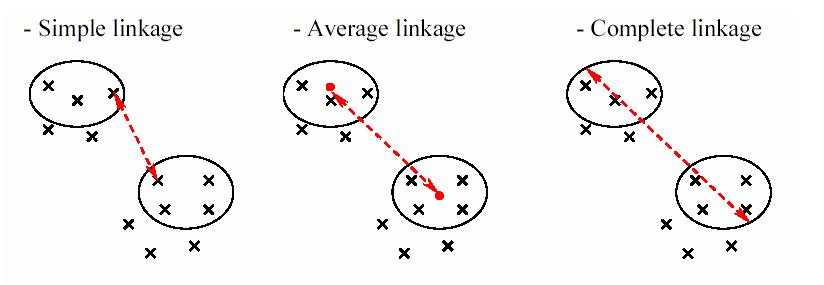
\includegraphics[width = 100mm]{linkages.jpg}
	\caption{Differenze fra i vari tipi di funzioni distanza}
	\label{linkages}
\end{figure}

\subsection{Graph Clustering}
Un grafo è una coppia ordinata $ G = (V, E)$ di insiemi, con $V$ insieme dei nodi ed $E$ insieme degli archi, tali che gli elementi di $E$ siano coppie di elementi da $V$ da $ E \subseteq V\times V$ segue in particolare che  $|E|\le |V|^2$.
\\\\
I grafi sono oggetti discreti che permettono di schematizzare una grande varietà di situazioni e di processi e spesso di consentirne delle analisi in termini quantitativi e algoritmici.
\\\\
Nello studio di reti complesse, è possibile trovare gruppi di nodi fortemente connessi, che possono essere raggruppati in comunità (potenzialmente sovrapposte). Questa disomogeneità di connessioni suggerisce che esiste una certa divisione naturale all’interno della rete. Nel caso particolare di strutture non sovrapposte, la ricerca di comunità implica la divisione della rete in gruppi di nodi con fortemente connessi internamente e connessioni sparse fra i gruppi.
Una definizione più generale è basata sul principio che coppie di nodi sono più probabilmente connessi se fanno parte della stessa comunità, e meno probabilmente connessi se non condividono la stessa comunità.
\\\\
Le comunità sono molto comuni all’interno delle reti. Le reti sociali includono gruppi di comunità che condividono la posizione, gli interessi, l’occupazione ecc. Essere in grado di individuare queste sotto-strutture all’interno di una rete può fornire indizi  su come come funziona la rete in considerazione o la topologia che influenza i nodi. Questi indizi possono essere utili per implementare algoritmi sui grafi. Molti metodi di community detection sono stati sviluppati con diversi livelli di successo.

\subsubsection{Minimum-cut method}
In questo metodo, la rete è divisa in un numero predeterminato di parti, generalmente della stessa grandezza, scelte in modo che il numero degli archi tra i gruppi è minimizzato. Questo metodo funziona bene in molte applicazioni per le quali è stato ideato, ma non è la scelta migliore per scovare comunità in reti generali, dato che troverà comunità indistintamente dal fatto che queste ci siano o meno e troverà solo un numero fissato di comunità.

\subsubsection{Hierachical-clustering}
Un altro metodo per scovare sotto-strutture conesse nelle reti viene effettuato tramite algoritmi di clustering gerarchico. Con questo approccio si definisce una misura di similarità fra coppie di nodi. Misure comunemente usate sono la coseno similarità, l’indice di Jaccard e la distanza di Hamming fra le righe della matrice di adiacenza. Poi i gruppi di nodi simili vengono raggruppati in comunità.

\subsubsection{Girvan-newman algorithm}
Un altro algoritmo molto utilizzato è quello di Girvan–Newman. Questo algoritmo identifica all’interno della rete, gli archi che uniscono community diverse e li rimuove, isolandole. L’identificazione di tali archi è effettuata applicando una misura nota della teoria dei grafi: la \textbf{betweenness centrality}. Questa assegna un valore ad ogni arco, che è alto tanto più l’arco è attraversato nel cammino più breve (geodesico) che collega due qualsiasi nodi della rete.
\begin{figure}[htb]
	\centering
	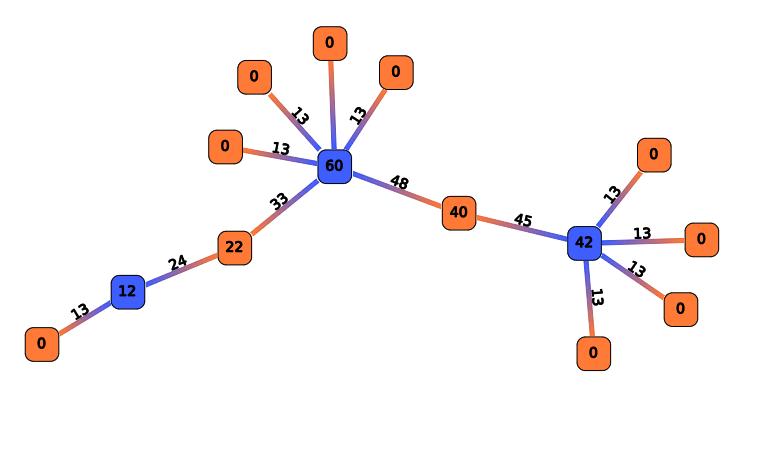
\includegraphics[width = 100mm]{betweenness.png}
	\caption{Betweenneess centrality score}
	\label{betweenness}
\end{figure}

\subsubsection{Modularity maximization}
La modularità è una misura che viene attribuita al grafo.  Questa compara la densità all’interno dei cluster con la densità fra di essi. Indica una certa divisione intrinseca e viene utilizzata per conoscere “quanto“ un grafo è separato.
\\\\
Nonostante i suoi svantaggi uno dei metodi più utilizzati per il community detection è la massimizzazione della modularità. Questo approccio scova strutture connesse tramite la ricerca della miglior divisione di una rete in modo che la modularità risulti massimizzata. 
\\\\
Dato che effettuare un confronto su tutte le possibili combinazioni è solitamente impraticabile, gli algoritmi di questa famiglia si basano su metodi di ottimizzazione approssimati quali algoritmi greedy, cioè che cercano di ottenere una soluzione ottima da un punto di vista globale attraverso la scelta della soluzione considerata migliore ad ogni passo locale. Un famoso approccio di questo tipo è il metodo Louvain, che ottimizza le community locali iterativamente, fin quando la modularità globale non può più essere migliorata. 
\\\\
L’accuratezza di questi algoritmi, comunque, è dibattuta, in quanto è stato dimostrato che molte volte fallisce nell’individuare cluster più piccola di una certa soglia, dipendente dalla grandezza della rete. 
\begin{figure}[htb]
	\centering
	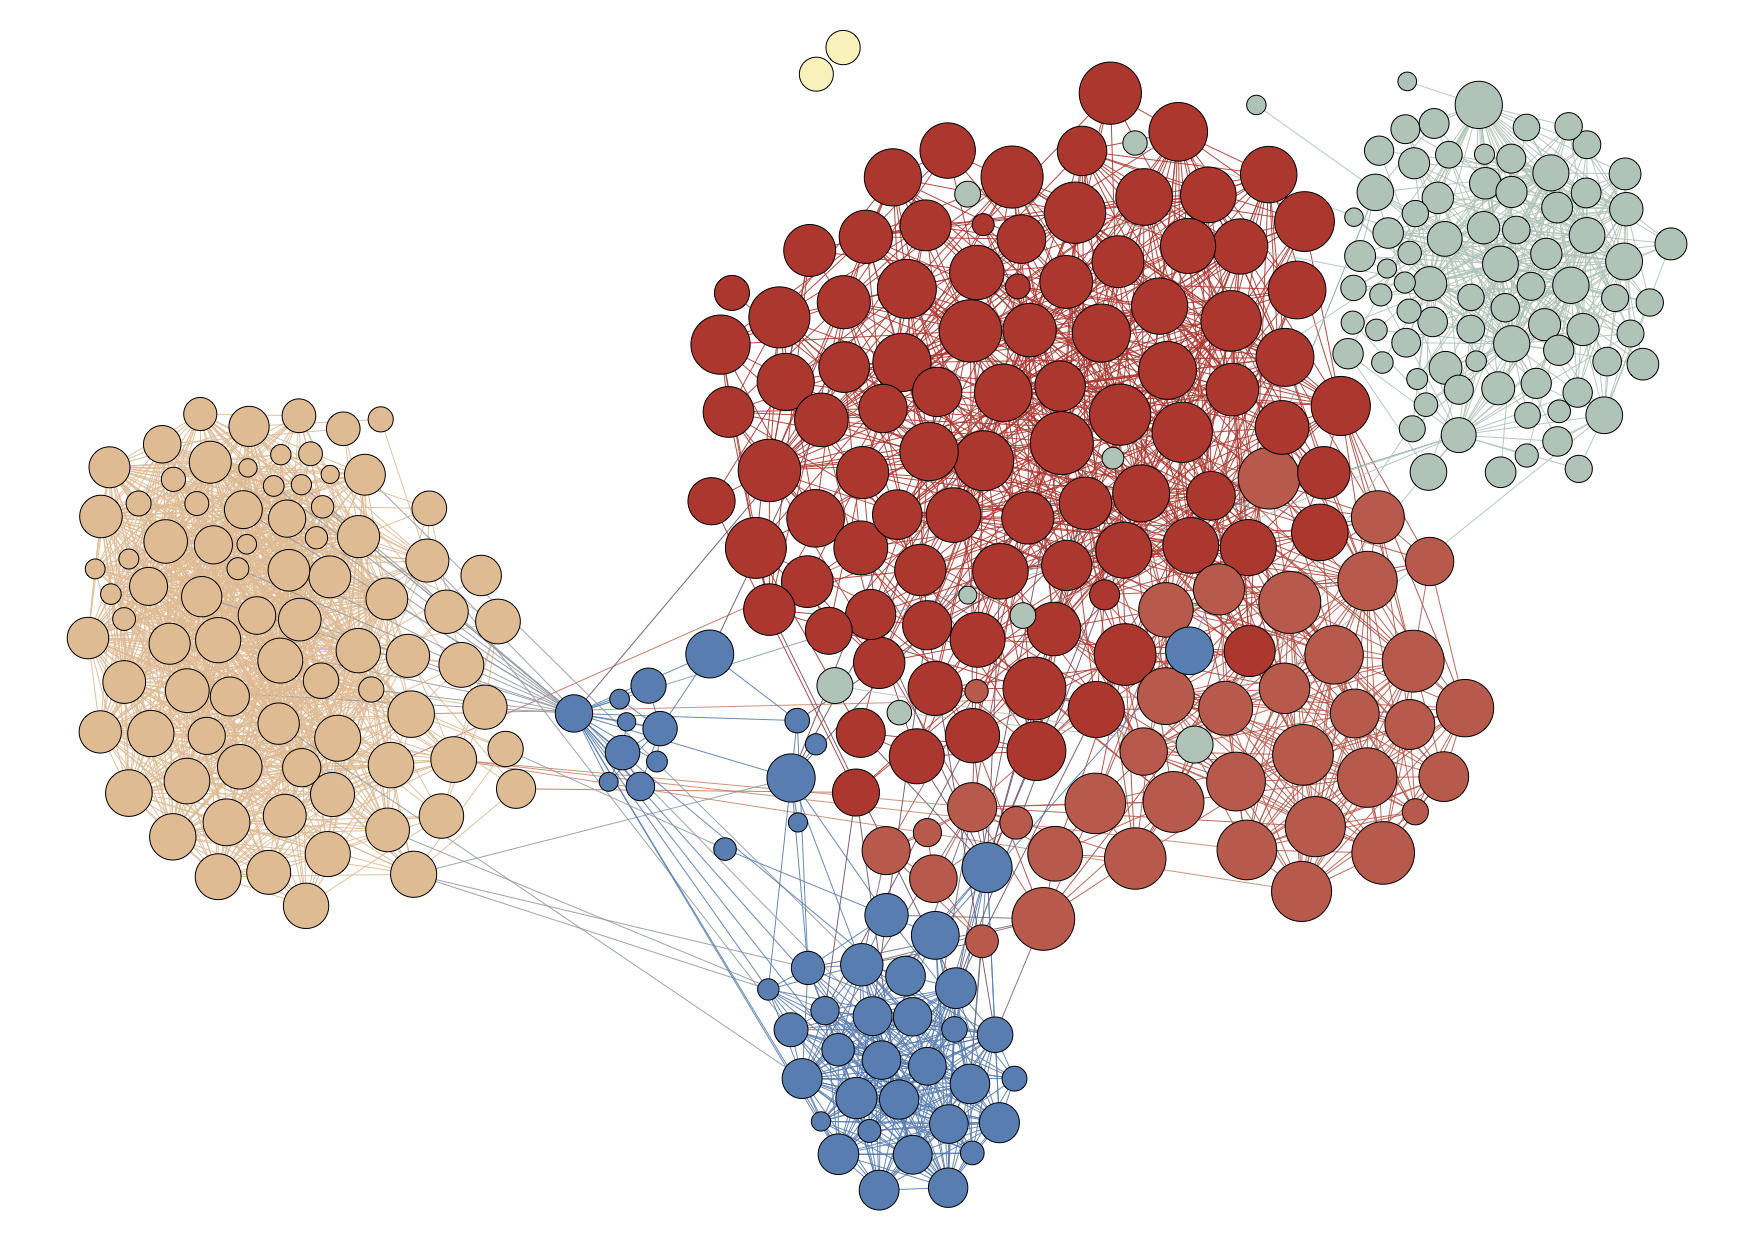
\includegraphics[width = 100mm]{modularity.png}
	\caption{Modularity score}
	\label{modularity}
\end{figure}
\subsubsection{Clique-based methods}
Le cricche (cliques) sono sottografi dove ogni nodo è collegato con ogni altro nodo nella cricca. Dato che i nodi non possono essere più connessi di così, non è sorprendente che ci siano molti metodi in community detection che si basano su questo approccio. È da notare che dato che un nodo può far parte di più di una cricca, quindi può far parte di più community contemporaneamente, questi metodi restituiscono strutture sovrapposte. 
Un approccio consiste nel trovare cricche tali che non siano sottografi di altre cricche. Un classico algoritmo per scovare tali strutture è quello di Bron-Kerbosch.



\subsection{Vector Clustering}
Gli algoritmi di clustering in uno spazio vettoriale seguono un altro approccio. Qui viene preso in considerazione la vicinanza (o la distanza) degli elementi rappresentati come punti su un iperpiano. Il feature vector associato può avere grandi dimensioni e può essere ottenuto utilizzando diverse metodologie, dipendentemente dal tipo di dato eleborato. 

\subsubsection{Hierarchical Clustering}
Anche qui il clustering gerarchico è molto utilizzato, seguendo un approccio divisivo (top-down) o agglomerativo (bottom-up), l’idea è quella di unire (o separare) elementi in base alla loro vicinanza, seguendo uno degli approcci già descritti, costruendo così una struttura chiamata dendrogramma che raggruppa gli elementi ad ogni livello. La differenza risiede nel come viene calcolata la distanza.

\subsubsection{Centroid-based clustering}
Nell’approccio basato sui centroidi, i cluster sonorappresentati da un vettore centrale, che non è neccessariamente un membro del dataset. Quando il numero dei cluster è prefissato ad un numero k, la seguente definizione formale può essere applicata: vengono definiti k centroidi e si prosegue assegnando ogni elemento al centroide più vicino, tale che il quadrato delle distanze dal cluster è minimizzato. Molti algoritmi di questa famiglia richiedono che il parametro k sia stabilito in precedenza, che è il loro più grande svantaggio. Inoltre solitamente vengono trovati cluster di grandezza simile, dato che verrà assegnato un elemento al centroide più vicino. Questi metodi partizionano lo spazio dei dati in una struttura conosciuta come diagramma di Voronoi.
\begin{figure}[htb]
	\centering
	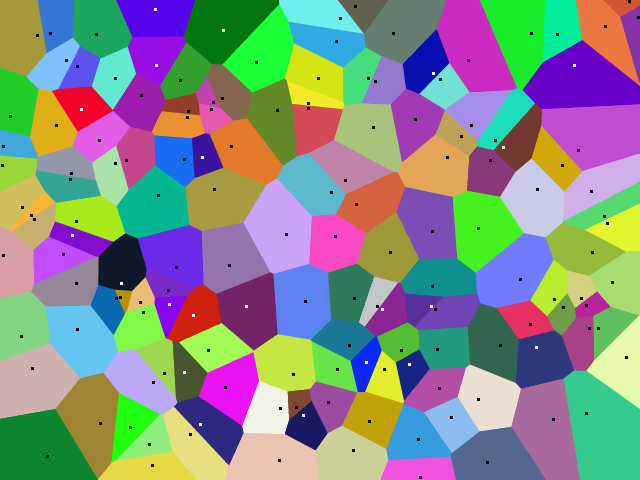
\includegraphics[width = 130mm]{voronoi.png}
	\caption{Diagramma di Voronoi}
	\label{voronoi}
\end{figure}
Nonostante questo, rimangono tra degli approcci più utilizzati ed efficaci. Da notare anche la somiglianza concettuale con l’algoritmo di classificazione KNN (k nearest neighbor).

\subsubsection{Distribution-based clustering}
Il raggruppamento avviene analizzando l'intorno di ogni punto dello spazio. In particolare, viene considerata la densità di punti in un intorno di raggio fissato. Si basano sul considerare collegati due punti che si trovano all’interno di una certa distanza limite.
I cluster sono definiti come aree con più alta densità rispetto al resto del dataset. Elementi in un area meno denso sono spesso considerati rumore, quindi come non facenti parte di nessun cluster.
\\\\
Uno degli svantaggi di questi algoritmi è che si aspettano un certo tipo di densità comune a tutti i cluster. Inoltre non eccellono nel scovare cluster presenti in molti dati del mondo reale.

\subsubsection{Document Clustering}
Agisce sempre nello spazio vettoriale, si differenzia principalmente nelle operazioni di pre-processing finalizzate ad ottenere un feature vector utilizzabile. 
Un approccio efficace consiste nel rappresentare i documenti come vettori dove ogni dimensione rappresenta la frequenza di occorrenza di una parola del vocabolario, un insieme di parole precedentemente costruito utilizzando tutte le parole del corpus. 
\begin{figure}[htb]
	\centering
	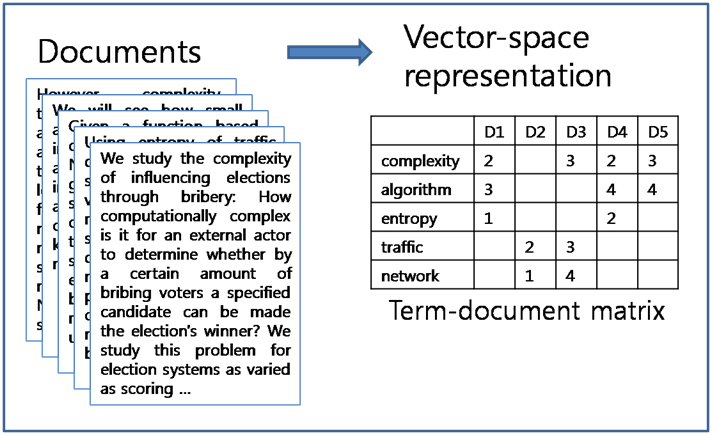
\includegraphics[width = 100mm]{tdm.png}
	\caption{Matrice termini-documenti. Ogni riga rappresenta un singolo termine ed ogni colonna rappresenta un singolo documento}
	\label{tdm}
\end{figure}

\paragraph{Term-Frequency (TF)}misura quante volte un termine appare in un documento. Dato che ogni documento ha lunghezza differente, è possibile che un termina possa apparire molte più volte nei documenti più lunghi che in quelli più corti. Quindi può essere necessario  dividere la frequenza dei termini per documenti aventi la stessa lunghezza.

\paragraph{Inverse-Document-Frequency (IDF)}un altro aspetto da considerare è a frequenza di un termine in un documento relativamente alla sua presenza globale in tutto il corpus. Tenendo in considerazione solo la frequenza di occorrenza tutti i termini sono considerati ugulamente importanti. Termini che appaiono molte volte in un documento ma meno volte in tutto il corpus potrebbero essere molto più significativi per quel specifico documento e portare molta più informazione, quindi tendono ad essere più importanti. Così come i termini che appaiono molte volte in tutti i dcoumenti del corpus sono spesso poco rilevanti e considerati inutili (stopwords).
\begin{equation}
	idf_i = \log \frac{|D|}{|\left \{ d : t_i \in d \right \}|}
\end{equation}
dove $ |D| $ è il numero di documenti nella collezione, mentre il denominatore è il numero di documenti che contengono il termine $t_i$.
Tale funzione aumenta proporzionalmente al numero di volte che il termine è contenuto nel documento, ma cresce in maniera inversamente proporzionale con la frequenza del termine nella collezione. L'idea alla base di questo comportamento è di dare più importanza ai termini che compaiono nel documento, ma che in generale sono poco frequenti.
\\\\
Altre tecniche utilizzate nel clustering sui documenti sono
\paragraph{LSI} il \textbf{Latent Semantic Indexing} è un metodo di indicizzazione e reperimento che usa una tecnica matematica chiamata decomposizione a valori singolari (SVD) per identificare pattern nelle relazioni tra i termini e i concetti contenuti in una colezione non strutturata di testo. La LSI è basata sul principio che parole che sono usate nello stesso contesto tendono ad avere significato simile. Chiamata così per la sua abilità di correlare semanticamente termini correlati che sono nascosti (latenti) in grandi collezioni testuali. La SVD può venire troncata per task di dimensionality reduction, in modo da diminuire la dimensione del vettore mantenendo comunque il significato.

\paragraph{Coseno similarità} una euristica per la misurazione della similitudine tra due vettori effettuata calcolando il coseno tra di loro. Dati due vettori di attributi numerici, $A$ e $B$, il livello di similarità tra di loro è espresso utilizzando la formula
\begin{equation}
	similarity = \cos \theta = \frac{A\cdot B}{||A||||B||}
\end{equation}
In base alla definizione del coseno, dati due vettori si otterrà sempre un valore di similitudine compreso tra $-1$ e $+1$, dove $-1$ indica una corrispondenza esatta ma opposta (ossia un vettore contiene l'opposto dei valori presenti nell'altro) e $+1$ indica due vettori uguali.
Nel caso dell'analisi dei testi, poiché le frequenze dei termini sono sempre valori positivi, si otterranno valori che vanno da 0 a $+1$, dove $+1$ indica che le parole contenute nei due testi sono le stesse (ma non necessariamente nello stesso ordine) e $0$ che non c'è nessuna parola che appare in entrambi.

\subsection{Clustering delle pagine Web}
In questa sezione si parlerà della soluzione proposta come alternativa alle normali tecniche di clustering delle pagine Web basate esclusivamente sul contenuto testuale. Infatti il fulcro del sistema è basato su metodologie nate nel campo del \textbf{Natural Language Processing} ma applicate nel contesto Web, in modo da aggiungere ulteriore informazione utile. Qui sarà approfondita l'idea alla base del lavoro svolto e le diverse opzioni che l'algoritmo mette a disposizione. 
L'algoritmo prende in input il grafo di un sito Web e le sequenze di Random Walk generate restituisce rappresentazioni vettoriali per ogni pagina.
La fase di sperimentazione vera e propria sarà approfondita nel capitolo successivo.

\subsection{Algoritmi utilizzati}
Vengono riportati di seguito gli algoritmi di clustering testati sul dataset generato. L'obiettivo della tesi comunque non è verificare la validità di questi ma verificare se la soluzione proposta rappresenti un miglioramento ed un possibile alternativa alle soluzioni più usate e consolidate nell'ambito del clustering di pagine Web.
\begin{itemize}
\item \textbf{WalkTrap}
È un approccio basato su Random Walk. L'idea generale è che se vengono generati dei Random Walk sul grafo, i percorsi rimarrano probabilmente all'interno della stessa comunità perchè ci sono meno archi che congiungono comunità diverse. 
\\
L'algoritmo esegue piccoli Random Walk (dipendente da un parametro in input) è usa i risultati per fondere comunità diverse in maniera bottom-up. Tagliando il dendrogramma risultante ad una certa altezza è possibile ricevere il numero di cluster desiderati.

\item \textbf{Fastgreedy}
È un approccio gerarchico bottom-up. Cerca di ottimizzare una funzione di modularità in maniera greedy, euristica attuata effettuando la scelta migliore con le informazioni in possesso ad ogni iterazione.
Inizialmente ogni nodo è una comunità separata e ricorsivamente si procede ad unire i nodi in modo che la fusione porti al massimo aumento di modularità rispetto al valore corrente. 
\\
L'algoritmo finisce quando non è più possibile aumentare la modularità. È un metodo veloce, solitamente usato come primo approccio perchè non ha parametri da modificare.
\item \textbf{K-Means}
Divide il dataset in un numero prefissato $k$ di cluster. Inizialmente vengono scelti casualmente $k$ punti, non necessariamente facenti parte del dataset, chiamati centroidi. Si procede assegnando ogni data point al centroide più vicino e ricalcolando il centroide sulla media aritmetica dei punti contiene. 
\\
Questo processo di assegnazione dei data point e ricalcolo dei centroidi continua fino a quando non avvengono più assegnazioni. I $k$ cluster risultanti saranno quelli restituiti. Anche questo algoritmo rappresenta spesso il punto di partenza nell'analisi di un dataset, in quanto molto spesso porta a buoni risultati ma ha come svantaggio il dover sapere a priori il numero di cluster desiderati.

\item \textbf{DBSCAN}
Deriva da \textit{Density-Based Spatial Clustering of Applications with Noise} è un algortimo basato sulla densità, connettendo regioni di punti con densità sufficientemente alta. Fondamentalmente, un punto $q$  è direttamente raggiungibile da un punto $p$ se non viene superata una data distanza $\epsilon$ e se $p$ è circondato da un numero sufficiente di punti, allora $p$ e $q$ possono essere considerati parti di un cluster. 
\\
Si può affermare che $q$ è density-reachable da $p$ se c'è una sequenza $p_1, p_2,  \ldots, p_n$ di punti con $p_1 = p$ e $p_n = q$ dove ogni $p_{i+1}$ è density-reachable direttamente da $p_i$. Da notare che la relazione density-reachable non è simmetrica (dato che $q$ potrebbe situarsi su una periferia del cluster, avendo un numero insufficiente di vicini per considerarlo un elemento genuino del cluster). Di conseguenza la nozione density-connected diventa: due punti $p$ e $q$ sono density-connected se c'è un punto $o$ tale che sia $o$ e $p$ che $o$ e $q$ sono density-reachable.
\\
Un cluster, che è un sotto-insieme dei punti del database, soddisfa due proprietà:

\textit{i)}Tutti i punti all'interno del cluster sono mutualmente density-connected.
\textit{ii)}Se un punto è density-connected a un altro punto del cluster, anch'esso è parte del cluster.

\item \textbf{HDBSCAN}
Deriva da \textit{Hierarchical Density-Based Spatial Clustering of Applications with Noise}~\cite{Campello15}. Applica DBSCAN variando il valore dell $\epsilon$ ed integra i risultati restituendo cluster che stabilizzano meglio tale valore.
\\
Questo permette ad HDBSCAN di trovare cluster con densità diversa, principale svantaggio di DBSCAN.
\end{itemize}
